\documentclass[conference]{IEEEtran}
\usepackage{amsmath,amssymb}
\usepackage{graphicx}
\usepackage{booktabs}
\usepackage{multirow}
\usepackage{array}
\usepackage{cite}
\usepackage{url}
\usepackage{xcolor}
\usepackage{stfloats}
\usepackage{float}
\graphicspath{{figures/}}

\title{Support-Constrained Concept Reachability for Cognitive Diagnosis under Concept Evidence Gaps}

\author{
\IEEEauthorblockN{Anonymous Author(s)}
\IEEEauthorblockA{Anonymous Affiliation\\
Email: anonymous@example.com}
}

\begin{document}
\maketitle

\begin{abstract}
Cognitive diagnosis estimates students' mastery of knowledge concepts from response histories. From an educational measurement perspective, diagnosis should connect historical responses with the target concept estimate. Existing neural and graph-based cognitive diagnosis models usually rely on student--exercise responses and Q-matrices, but a target concept in the current exercise may not be directly covered by a student's history. This creates a concept evidence gap between observed responses and the mastery state to be diagnosed. We propose a concept reachability framework with two components: Concept Reachability Graph (CRG) and Learner-Conditioned Reachability Filter (LCRF). CRG constructs a concept relation graph from training-stage item co-occurrence, sequence transition, and self-retention relations, and returns a fixed support set for each target concept. LCRF assigns posterior weights to support concepts using learner mastery, recent performance, and historical counts. Experiments on three real-world datasets show competitive prediction performance and indicate that CRG-LCRF is particularly useful in coverage-conditioned settings where direct concept coverage is limited but candidate route support exists.
\end{abstract}

\begin{IEEEkeywords}
Cognitive diagnosis, concept evidence gap, concept reachability graph, support-constrained diagnosis, learner-conditioned filtering
\end{IEEEkeywords}

\section{Introduction}
Cognitive diagnosis (CD) estimates learners' mastery of knowledge concepts from historical response logs and exercise--concept relations. Its outputs support personalized practice, remediation, learning-path planning, and adaptive testing. From an educational measurement perspective, diagnosis is more than score prediction: the predicted response should be connected to concepts and previous observations that support the target mastery estimate~\cite{pellegrino2001knowing,mislevy2003structure}. This requirement becomes challenging when the target concept of a query exercise is weakly covered, or not covered at all, by the learner's previous interactions.

In real learning platforms, student histories often cover only part of the concept space. A target concept required by the current query exercise may never appear in the learner's past interactions, or may have only a few direct observations. The model can still output a probability, but the connection from historical responses to the target concept becomes indirect. We call this phenomenon the \emph{concept evidence gap}: the target concept needs to be diagnosed, while the learner history lacks direct concept coverage and the model must seek support from related historical concepts and concept relations observed in training logs.

This setting differs from general short-history or cold-start diagnosis. A learner may have a long response history while still lacking observations on the particular concept required by the current exercise. Conversely, a short history may still contain direct observations on the target concept. The key condition is therefore not only the length of the history, but whether the target concept can be connected to the learner's observed concepts through relations available in the training logs.

Existing neural CDMs and graph CDMs mainly exploit response logs, Q-matrices, or heterogeneous graph propagation, but they often compress two different questions into a single representation-learning process. The first question is \emph{support construction}: when the target concept is absent from the learner history, can the model find candidate support concepts from related historical concepts through concept relations observed in training logs? The second question is \emph{learner-state filtering}: given the same candidate support, which support concepts are reliable for the current learner's mastery state, recent performance, and historical reliability?

This distinction matters in real learning platforms. Item-level concept co-occurrence alone can degenerate on single-concept datasets, leaving few connections between historical concepts and the target concept. Pure student or item embeddings may still fit response accuracy, but they do not clearly indicate which historical concepts support the target diagnosis. From an educational diagnosis perspective, connecting historical concepts to a target concept provides prior performance support for the current mastery judgment. Such support may come from within-exercise co-occurrence or from empirical learning order observed in response logs. This motivates a mechanism that combines concept support construction with learner-state filtering.

The proposed setting also changes how model analysis should be organized. Average prediction performance remains necessary, but it does not show whether the model addresses the target condition. A model may improve AUC by better fitting frequent concepts while still failing when the query concept is not directly observed in the learner history. Therefore, our evaluation follows the same problem structure as the method: we first check whether concept route support exists, then test whether the route support can retrieve target concepts, and finally analyze how prediction changes when support concepts or learner-state inputs are perturbed.

We propose a two-stage CRG/LCRF framework. CRG constructs a global concept roadmap from training-stage concept relations and returns a fixed support set for each target concept. LCRF then assigns learner-conditioned posterior weights over that support using mastery, recent performance, and historical counts. In this way, CRG addresses support construction, while LCRF addresses learner-conditioned filtering over the constructed support.

\begin{figure*}[!t]
  \centering
  
\includegraphics[width=0.96\textwidth]{fig1_problem_concept_evidence_gap.png}
  \caption{Concept evidence gap. The target concept may not be directly covered by the learner history. CRG retrieves candidate support concepts from training-stage concept relations, and LCRF reweights posterior weights within the fixed support according to learner state.}
  \label{fig:concept-gap}
\end{figure*}

Figure~\ref{fig:concept-gap} illustrates the problem. Historical concepts provide limited observed signals, but the query concept \(c_q\) may be absent from the learner's historical concept set. CRG connects historical concepts to the target concept through empirical relations in training logs. Sequence transition denotes empirical learning order rather than a causal curriculum relation. LCRF then assigns posterior weights within the CRG-defined fixed support. The design is consistent with adaptive learning support: a globally available support concept becomes more useful when it matches the current learner state.

Our contributions are summarized as follows.
\begin{itemize}
  \item We formulate the concept evidence gap as a support construction problem in cognitive diagnosis.
  \item We propose CRG, which constructs concept support from training-stage item co-occurrence, sequence transition, and self-retention evidence.
  \item We propose LCRF, which reweights posterior weights over the fixed CRG support using learner state.
  \item We evaluate CRG-LCRF through prediction performance, route retrieval, support perturbation, learner-state counterfactuals, and same-query case analysis, showing how route construction and learner-conditioned filtering contribute under sparse concept coverage.
\end{itemize}

\section{Related Work}
\subsection{Cognitive Diagnosis Models}
Traditional CD models are rooted in psychometrics, such as IRT, MIRT, and DINA~\cite{lord1980irt,reckase2009mirt,delatorre2009dina,templin2006cdm}. They describe learner ability, item difficulty, attribute mastery, and responses with predefined interaction functions. FuzzyCD extends this line by modeling fuzzy mastery states~\cite{liu2018fuzzycd}. Neural CDMs replace fixed response functions with flexible neural interactions and improve prediction on large-scale educational logs~\cite{wang2020ncdm}. NCDM and KaNCD map students, exercises, and concepts into continuous spaces~\cite{wang2020ncdm,wang2022kscd}. These models usually depend on the Q-matrix and observed responses to update concept representations. When the target concept is absent from a learner's history, they may still fit response probability through global parameters or embeddings, but they do not explicitly identify which related concepts support the target estimate.

The distinction between response prediction and concept-level support is important for diagnostic interpretation. A high predicted probability can be produced by student ability, item easiness, or latent embeddings, but the diagnosis is less informative if the model cannot relate the prediction to concepts the learner has practiced. CRG-LCRF keeps the standard prediction goal, while adding an explicit route-support layer between historical concepts and the target concept.

This route-support view does not replace the Q-matrix. The Q-matrix still defines which concepts are required by each exercise. The missing part is learner-specific: the target concept may be present in the Q-matrix but absent from the learner's own history. Therefore, our method operates after the exercise--concept relation is known, and asks how the target concept can be supported by the learner's previous concept observations.

\subsection{Graph-Based Cognitive Diagnosis}
Graph-based CD models propagate information on student--exercise graphs, exercise--concept graphs, or heterogeneous graphs. Graph structures can improve representations and capture dependencies among students, exercises, and concepts~\cite{kipf2017gcn,velickovic2018gat,hamilton2017graphsage,he2020lightgcn,su2022gcdm}. RCD, SCD, and ORCDF further exploit relation-aware or graph-based structures to improve representation learning~\cite{gao2021rcd,wang2023scd,qian2024orcdf}. Such propagation is useful when neighboring nodes carry reliable diagnostic information. Recent work also shows that graph edges can be heterogeneous or uncertain, because correct and incorrect responses may have different meanings and noisy edges may mislead representation learning~\cite{wang2024uncertaintycd,shao2025isgcd,zhang2026ncdla}. Our setting focuses on a complementary issue: even when the graph is constructed from training logs, the target concept of a query may not be directly observed in the learner history. CRG therefore constructs concept-level route support rather than relying only on generic graph propagation.

Another difference is the granularity of the relation being used. Student--exercise graphs mainly capture interaction exposure, and exercise--concept graphs mainly follow the Q-matrix. They are valuable for representation learning, but they do not directly answer whether the target concept can be supported by concepts that appeared in the learner's history. CRG operates at the concept level and uses item co-occurrence, temporal order, and self-retention as separate route sources, which makes the support construction step explicit.

The separation between route construction and learner filtering also differs from attention-based graph aggregation. Attention weights learned inside a graph neural network may improve representation quality, but their candidate neighbors are often determined by the graph schema or learned embeddings. In CRG-LCRF, the candidate support is first determined by training-log concept relations, and only then reweighted by learner-state features. This ordering allows the analysis to ask whether the support itself is useful and whether learner-state filtering changes the posterior over that support.

\subsection{Sparse Evidence and Reliable Diagnosis}
Recent CD studies address data insufficiency from cold-start students or items, missing-not-at-random responses, noisy interactions, and unreliable graph edges. KCD and LRCD leverage language representations for cold-start, open-world, or cross-domain diagnosis~\cite{dong2025kcd,liu2025lrcd}. DBCD, HeckmanCD, and fairness-aware CD analyze selection bias, exposure bias, and counterfactual mechanisms in observed logs~\cite{yang2026dbcd,han2024heckmancd,zhang2024faircd,zhang2024causalcdf}. NCDLA and DisenGCD study robustness under noisy responses, Q-matrix errors, or unstable graph structures~\cite{zhang2026ncdla,yang2024disengcd}. Language learning and conversational diagnosis further broaden CD scenarios~\cite{ma2024languagecd,yao2026parld}. These settings are related to our problem, but not identical. Concept evidence gaps can occur even when the learner is not new and the history is not extremely short: the missing part is the direct coverage of the target concept, not necessarily the entire learner or item history.

Student-concept sparsity is especially relevant. A learner can answer many exercises while covering only a limited subset of concepts. Existing methods often treat this as a representation sparsity problem, using external text, graph propagation, or transfer learning to enrich embeddings. We instead focus on the query-level condition induced by this sparsity: for the current target concept, does the learner history provide direct observations, and if not, can related concepts provide a usable route?

\subsection{Educational Measurement and Adaptive Support}
Educational measurement treats assessment as inference from observable responses to latent student states~\cite{pellegrino2001knowing,mislevy2003structure}. Under this view, the absence of direct historical coverage for a target concept creates an indirect relation between previous responses and the current concept. Learning progression studies suggest that concept understanding may develop along empirically observable paths, but such paths should not be treated as deterministic causal relations~\cite{corcoran2009learning}. Adaptive support theories, including the zone of proximal development, scaffolding, and mastery learning, also suggest that available support should be adjusted according to the learner's current state~\cite{vygotsky1978mind,wood1976tutoring,bloom1968learning}. These ideas motivate our design at a high level: CRG constructs training-log-derived route support, and LCRF selects among that support according to learner-state features. We use these theories as interpretation guidance rather than as assumptions of causal concept relations.

This educational interpretation guides the scope of the claims. The framework predicts responses as other CDMs do, but its analysis emphasizes whether the prediction can be associated with concept-level support. A route found by CRG is treated as a candidate diagnostic support relation observed from data, and a route emphasized by LCRF is treated as a learner-conditioned weighting of that support.

\section{Problem Definition}
Let \(\mathcal{U}\), \(\mathcal{E}\), and \(\mathcal{C}\) denote students, exercises, and concepts. The Q-matrix specifies exercise--concept relations, and the response log \(\mathcal{R}\) consists of student, exercise, and binary response tuples. For learner \(u\) at time \(t\), \(H_{u,t}\) denotes concepts observed in the previous interactions.

We use two diagnostics to characterize the coverage condition of a query. Direct coverage \(D_{u,t}(c)\) indicates whether target concept \(c\) appears in \(H_{u,t}\). CRG reachability indicates whether the target concept admits candidate support concepts under the fixed CRG support \(S_A(c)\). When \(D_{u,t}(c)=0\), the learner has no direct historical performance on the target concept. If CRG reachability is still present, the target concept may be supported by related concepts in the learner history through training-stage concept relations.

For exercises involving multiple concepts, the query is considered weakly covered if at least one required concept lacks direct historical observations. We also use the query history count to describe how often the target concept has appeared before the query. These quantities describe the diagnostic condition of each event. They do not change the task input, the training objective, or the test set.

This definition is query-centered. A learner can be experienced at the platform level and still face a concept evidence gap on a particular exercise. Likewise, a concept may be frequent globally but rarely observed for a specific learner. The proposed diagnostics therefore describe the relation between a learner's own history and the target concept of the current query, rather than only global dataset sparsity.

The model is trained and evaluated on all response instances. Subgroup analysis examines how the model behaves in direct-unseen and bridgeable conditions. The concept reachability graph is estimated from training-stage observable concept relations and is frozen during validation and testing.

\section{Concept Evidence Gap Phenomenon}
\begin{figure}[!t]
  \centering
  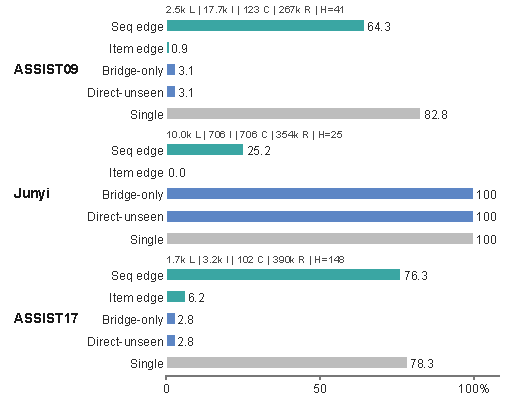
\includegraphics[width=0.98\columnwidth]{fig_dataset_evidence_profiles.pdf}
  \caption{Dataset coverage-gap profiles. Blue bars show direct coverage conditions, teal bars show available route sources, and gray bars show the single-concept exercise ratio. The compact header in each card reports learners (L), items (I), concepts (C), responses (R), and median history length (H).}
  \label{fig:dataset-profile}
\end{figure}

Figure~\ref{fig:dataset-profile} summarizes the dataset scale and coverage-gap statistics, and serves as a prevalence analysis of the target problem. Direct-unseen rate denotes the proportion of test queries whose target concept has not appeared in the learner history. Bridge-only rate denotes the proportion of these direct-unseen queries whose target concept can still be connected to the learner history through CRG support. The two rates characterize whether direct concept coverage is missing and whether candidate support concepts still exist.

The other columns describe which relation sources are available. Item-edge density reflects whether concept relations can be obtained from exercises containing multiple concepts. For example, an exercise may require both equation transposition and solving a linear equation, giving a within-exercise co-occurrence relation between the two concepts. Sequence-edge density reflects whether training logs provide empirical transitions between concepts across consecutive learner interactions. Junyi represents a sequence-route regime: all exercises are single-concept, so item co-occurrence is unavailable, but a large fraction of target concepts can still be connected through training-log transitions. ASSIST09 and ASSIST17 contain sparse item co-occurrence and dense sequence transitions, making them closer to mixed-relation CD benchmarks.

These observations motivate a route-based support constructor. A useful concept roadmap should not rely solely on within-item co-occurrence, and its sequence relations should be interpreted as empirical transitions observed in learning logs rather than curriculum constraints.

\section{Method}
\subsection{Overview}
CRG constructs a global concept reachability graph and returns a fixed support set. LCRF performs learner-conditioned posterior filtering over the same support. The computation is organized as four steps. First, training-stage concept relations estimate \(A_{\mathrm{CRG}}\). Second, the row \(A_{\mathrm{CRG}}(c,:)\) selects the fixed support \(S_A(c)\) for query concept \(c\). Third, LCRF combines \(S_A(c)\) with learner state \(\mathbf{x}_{u,t}\) to produce \(P_{\mathrm{LCRF}}(k|u,t,c)\). Finally, the diagnosis head uses the posterior distribution to predict \(\hat r_{u,e}\).

\begin{figure*}[!t]
  \centering
  
\includegraphics[width=0.96\textwidth]{fig2_crg_lcrf_architecture.png}
  \caption{CRG/LCRF framework. CRG constructs a global concept reachability graph from training-stage item co-occurrence, sequence transition, and self-retention evidence, and returns a fixed support for the target concept. LCRF reweights posterior weights over support concepts using learner mastery, recent performance, and historical counts.}
  \label{fig:framework}
\end{figure*}

As shown in Figure~\ref{fig:framework}, CRG uses training-log relations to build a concept reachability graph and returns a fixed support \(S_A(c)\) for the query concept. LCRF uses learner-state features to personalize posterior weights within the same support. The pipeline separates two operations that are often entangled in representation learning: CRG determines which support concepts are available for a target concept, while LCRF determines how strongly each support concept should contribute for the current learner.

This separation also clarifies the ablation design. Removing CRG removes the route-support substrate, so the model loses the concept candidates used by the local filter. Removing LCRF keeps the global support but removes the learner-state correction over that support. The two variants therefore correspond to different parts of the pipeline rather than two arbitrary parameter deletions.

\subsection{Concept Reachability Graph}
For concepts \(a,b\), item co-occurrence, sequence transition, and self-retention evidence are
\[
\begin{aligned}
M^{item}_{a,b}
&=\sum_{e\in \mathcal{E}^{tr}} Q_{e,a}Q_{e,b}\mathbb{I}[a\neq b],\\
M^{seq}_{a,b}
&=\sum_{u,t}
\mathbb{I}[a\in C(e_{u,t})]\,
\mathbb{I}[b\in C(e_{u,t+1})],\\
M^{self}_{a,b}
&=\mathbb{I}[a=b].
\end{aligned}
\]
\(M^{item}\) is useful when exercises involve multiple concepts. Self-retention is modeled separately by \(M^{self}\), so item co-occurrence only captures within-exercise relations between distinct concepts. \(M^{seq}\) denotes empirical learning order observed in training logs; this interpretation is consistent with learning progression research that emphasizes observed developmental paths without assuming a single causal ordering~\cite{corcoran2009learning}. \(M^{self}\) keeps concept-specific state retention.

Connecting historical concepts to a target concept can be viewed as finding prior performance support for the current diagnosis; this support comes from related concepts practiced by the learner and empirical order in the training logs. CRG converts the three sources into comparable relation scores:
\[
\begin{aligned}
s_{item}(a,b)&=\lambda_{item}\phi(M^{item}_{a,b}),\\
s_{seq}(a,b)&=\lambda_{seq}\phi(M^{seq}_{a,b}),\\
s_{self}(a,b)&=\lambda_{self}M^{self}_{a,b}.
\end{aligned}
\]
The total relation score adds the receiver bias \(b_b\):
\[
s(a,b)=s_{item}(a,b)+s_{seq}(a,b)+s_{self}(a,b)+b_b .
\]
Before normalization, CRG first collects candidate concepts supported by at least one training-stage relation:
\[
\mathcal{N}(a)
=
\{b\mid
M^{item}_{a,b}
+M^{seq}_{a,b}
+M^{self}_{a,b}>0
\}.
\]
The row-normalized reachability graph is then computed over the candidate set:
\[
A_{\mathrm{CRG}}(a,b)
=
\operatorname{softmax}_{b\in \mathcal{N}(a)}
\left(s(a,b)/\tau\right).
\]
The temperature \(\tau\) controls the smoothness of relation weights. For a query concept \(c\), the fixed support is selected by top-\(K\) neighboring concepts:
\[
S_A(c)=
\operatorname{TopK}_{k\in \mathcal{N}(c)}
A_{\mathrm{CRG}}(c,k).
\]
Here \(\mathcal{N}(a)\) is the candidate concept set, and \(S_A(c)\) is the fixed support used by LCRF for target concept \(c\). The three relation sources play different roles: item co-occurrence captures concepts that appear in the same exercise, sequence transition captures empirical concept transitions in learner logs, and self-retention keeps the target concept itself as a possible support candidate when direct concept information exists.

\subsection{Learner-Conditioned Reachability Filter}
LCRF computes a learner-conditioned posterior over the fixed support. Inspired by scaffolding and the zone of proximal development, LCRF filters globally available support concepts into local support that better matches the current learner state~\cite{vygotsky1978mind,wood1976tutoring}.

The CRG relation probability is first converted into a prior logit:
\[
z^{prior}_{c,k}=\log A_{\mathrm{CRG}}(c,k).
\]
Learner state then contributes a local correction:
\[
\begin{aligned}
\Delta_{u,t,c,k}&=f_{\theta}(\mathbf{x}_{u,t,c,k}),\\
z^{state}_{u,t,c,k}&=\alpha_{u,t,c}\Delta_{u,t,c,k}.
\end{aligned}
\]
Here \(\mathbf{x}_{u,t,c,k}\) contains query and support mastery \(m\), recent performance \(\rho\), and historical count or reliability \(n\). The prior and state logits are combined and normalized over the fixed support:
\[
\begin{aligned}
z_{u,t,c,k}
&=z^{prior}_{c,k}+z^{state}_{u,t,c,k},\\
P_{\mathrm{LCRF}}(k|u,t,c)
&=\operatorname{softmax}_{k\in S_A(c)}(z_{u,t,c,k}).
\end{aligned}
\]
The prior logit preserves the global route strength from CRG, while the state correction adjusts this strength according to the learner. Thus, the same fixed support can lead to different posterior weights for different learners.
The posterior then aggregates mastery over support concepts:
\[
\begin{aligned}
\tilde{m}_{u,t}(c)=&
(1-\gamma)m_{u,t}(c)\\
&+\gamma
\sum_{k\in S_A(c)}
P_{\mathrm{LCRF}}(k|u,t,c)m_{u,t}(k).
\end{aligned}
\]
The interpolation coefficient \(\gamma\) controls how much the local support contributes to the target concept representation. If the learner has strong direct mastery information for the target concept, the first term can dominate. When direct concept information is limited, the second term allows route-neighbor mastery to contribute through the LCRF posterior. This aggregation is passed to the same prediction head used for all variants, so differences in the ablation study come from the support and filtering components rather than from a different output head.

\subsection{Prediction and Optimization}
The support-aware representation is fed into the diagnosis head to obtain \(\hat r_{u,e}\). The model is optimized by binary cross-entropy over training responses. In the ablation study, w/o CRG removes \(A_{\mathrm{CRG}}\) and the fixed support, while w/o LCRF removes the learner-state correction \(z^{state}_{u,t,c,k}\).

For multi-concept exercises, the support-aware mastery representation is computed for each required concept and combined by the diagnosis head. This keeps the prediction task aligned with the Q-matrix while allowing each target concept to receive its own route support. All relation statistics used by CRG are estimated before validation and testing, and the same frozen graph is used for all evaluation variants that retain CRG.

\section{Experiments}
The experiments are organized around the two operations introduced in the method. First, we report overall prediction performance to compare CRG-LCRF with representative CD baselines. Second, we examine route construction: dataset profiles describe whether direct coverage gaps occur, and retrieval experiments test whether CRG can recover target concepts or held-out concept transitions from training-log relations. Finally, we examine learner-conditioned filtering through ablation, support perturbation, learner-state counterfactuals, and same-query cases. This layout separates the existence of route support from its prediction-level use.

\subsection{Experimental Settings}
We use three public datasets: ASSIST09, Junyi, and ASSIST17~\cite{assistments2009,heffernan2017assistments,assistments2017,choi2020ednet}. ASSIST09 and ASSIST17 are common short names for the ASSISTments series, while Junyi is collected from a large online learning platform. Figure~\ref{fig:dataset-profile} reports the number of learners, exercises, concepts, response logs, and coverage statistics after preprocessing. All datasets use fixed train/validation/test splits. CRG is constructed from training-stage relations and frozen for validation and testing.

We report AUC, ACC, RMSE, and BCE. AUC reflects ranking quality and is the primary comparison metric in most CD benchmarks, while ACC and RMSE describe thresholded classification and calibration-related error. Baselines include psychometric models, neural CD models, graph-based CD models, and relation-aware CD models: IRT, DINA, NeuralCD, LightGCN, KaNCD, RCD, and SCD~\cite{lord1980irt,delatorre2009dina,wang2020ncdm,he2020lightgcn,wang2022kscd,gao2021rcd,wang2023scd}. The same data split and evaluation protocol are used for CRG-LCRF and all ablated variants.

\subsection{Overall Prediction Performance}
\begin{table}[H]
\centering
\caption{Overall prediction performance.}
\label{tab:main-performance}
\scriptsize
\setlength{\tabcolsep}{2.4pt}
\resizebox{\columnwidth}{!}{%
\begin{tabular}{llcccccc}
\toprule
\multirow{2}{*}{Category} & \multirow{2}{*}{Model} &
\multicolumn{2}{c}{ASSIST09} & \multicolumn{2}{c}{Junyi} & \multicolumn{2}{c}{ASSIST17}\\
\cmidrule(lr){3-4}\cmidrule(lr){5-6}\cmidrule(lr){7-8}
& & AUC & ACC & AUC & ACC & AUC & ACC\\
\midrule
Traditional \& Deep & IRT & 0.7415 & 0.7132 & 0.7789 & 0.7392 & 0.7238 & 0.6561\\
Traditional \& Deep & DINA & 0.7482 & 0.7158 & 0.7795 & 0.7421 & 0.7259 & 0.6625\\
Traditional \& Deep & NeuralCD & 0.7523 & 0.7228 & 0.7812 & 0.7472 & 0.7320 & 0.6700\\
Graph-based & LightGCN & 0.7593 & 0.7256 & 0.7832 & 0.7502 & 0.7512 & 0.6813\\
Graph-based & KaNCD & 0.7640 & 0.7315 & 0.7885 & 0.7556 & 0.7640 & 0.7315\\
Graph-based & RCD & 0.7685 & 0.7330 & 0.8087 & 0.7685 & 0.7676 & 0.6953\\
Disentangled & SCD & 0.7701 & 0.7321 & 0.8134 & 0.7726 & 0.7753 & 0.7028\\
\textbf{Ours} & \textbf{CRG-LCRF} & \textbf{0.7783} & \textbf{0.7407} & \textbf{0.8291} & 0.7688 & \textbf{0.7847} & \textbf{0.7151}\\
\bottomrule
\end{tabular}
}
\end{table}

Table~\ref{tab:main-performance} reports the overall prediction performance. CRG-LCRF obtains the best AUC on all three datasets. Its ACC is also competitive, although not always the highest, suggesting that the main gain is more clearly reflected in ranking-oriented prediction. Compared with the strongest baseline SCD, CRG-LCRF improves AUC by 0.0082 on ASSIST09, 0.0157 on Junyi, and 0.0094 on ASSIST17. These average results provide the overall performance basis, while the following analyses locate where the gains arise under sparse concept coverage.

\subsection{Diagnosis under Concept Evidence Gaps}
Figure~\ref{fig:dataset-profile} reports how often target concepts lack direct historical coverage. This subsection combines two problem-oriented analyses. History-to-query retrieval evaluates whether CRG can retrieve the current target concept from learner history concepts. Held-out transition retrieval evaluates whether training-log concept relations recover future concept transitions beyond self-only and random controls.

\begin{figure}[!t]
  \centering
  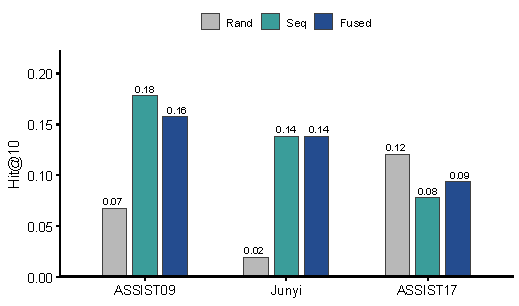
\includegraphics[width=0.98\columnwidth]{fig4_history_to_query_retrieval.pdf}
  \caption{History-to-query concept retrieval on direct-unseen-bridgeable samples. Seq-only and fused routes improve over random retrieval on ASSIST09 and Junyi. ASSIST17 is kept as a comparison case, where this retrieval setting is less favorable.}
  \label{fig:history-to-query}
\end{figure}

\begin{figure}[!t]
  \centering
  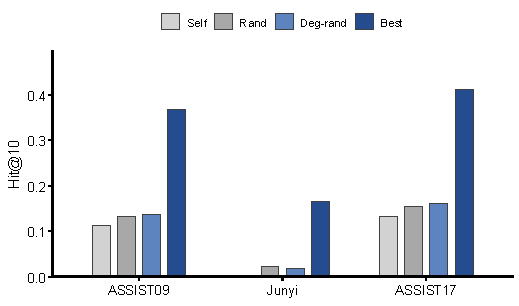
\includegraphics[width=0.98\columnwidth]{fig5_heldout_transition_retrieval.pdf}
  \caption{Held-out concept transition retrieval. Best CRG denotes the best-performing CRG route source for each dataset. This global retrieval task evaluates whether training-stage concept relations recover held-out concept transitions beyond self-only and random controls.}
  \label{fig:heldout-retrieval}
\end{figure}

Figure~\ref{fig:history-to-query} evaluates whether CRG can retrieve the current target concept from learner history concepts. On direct-unseen-bridgeable samples, random Hit@10 is 0.0673 on ASSIST09, while seq-only and fused CRG reach 0.1781 and 0.1574. On Junyi, random Hit@10 is 0.0191, while seq-only and fused CRG both reach 0.1379. These results indicate that training-log concept relations provide useful candidate support when direct target-concept history is absent. ASSIST17 does not show the same pattern in this history-to-query retrieval setting, so we keep it as a comparison case rather than a positive case for this specific task.

Figure~\ref{fig:heldout-retrieval} evaluates concept recovery at the global transition level. Seq-only and fused CRG outperform self-only and degree-random controls on ASSIST09, Junyi, and ASSIST17. This result supports the use of empirical sequence relations as concept support, especially when item co-occurrence is sparse or unavailable. The sequence relations are empirical associations from response logs and are not interpreted as causal curriculum rules. Together, the two retrieval figures separate two roles of CRG: retrieving the query concept from learner history in selected coverage-gap cases, and recovering held-out concept transitions from training-stage relations.

We also examine prediction behavior in coverage-conditioned subgroups without adding another main table. The pattern is dataset-dependent. On ASSIST09, Full has lower BCE than w/o CRG and w/o LCRF in direct-unseen-bridgeable, weak-direct-high-route, and high-route groups. On ASSIST17, the direct-unseen-bridgeable and high-route groups also show positive BCE improvements. On Junyi, the route retrieval signal is clearer than the prediction-level gain, which is consistent with Junyi being a route-construction regime rather than a strong learner-filtering case. These subgroup results suggest that the average AUC improvement in Table~\ref{tab:main-performance} should be read together with the availability of route support.

\subsection{Ablation Study}
\begin{table}[H]
\centering
\caption{Module ablation results.}
\label{tab:ablation}
\small
\setlength{\tabcolsep}{3.2pt}
\begin{tabular}{llccc}
\toprule
Dataset & Metric & Full & w/o CRG & w/o LCRF\\
\midrule
\multirow{3}{*}{ASSIST09}
& AUC  & \textbf{0.7783} & 0.7671 & 0.7634\\
& ACC  & \textbf{0.7407} & 0.7320 & 0.7309\\
& RMSE & \textbf{0.4178} & 0.4222 & 0.4247\\
\midrule
\multirow{3}{*}{Junyi}
& AUC  & \textbf{0.8291} & 0.8278 & 0.8286\\
& ACC  & 0.7688 & 0.7691 & \textbf{0.7701}\\
& RMSE & 0.4008 & 0.4011 & \textbf{0.3994}\\
\midrule
\multirow{3}{*}{ASSIST17}
& AUC  & \textbf{0.7847} & 0.7647 & 0.7829\\
& ACC  & \textbf{0.7151} & 0.6973 & 0.7132\\
& RMSE & \textbf{0.4321} & 0.4413 & 0.4359\\
\bottomrule
\end{tabular}
\end{table}

Table~\ref{tab:ablation} reports module ablations. Full denotes the complete model, w/o CRG removes the concept reachability graph, and w/o LCRF keeps CRG while removing learner-conditioned filtering.

The Full model obtains the highest AUC on ASSIST09 and ASSIST17. Removing CRG causes 1.12\% and 2.00\% AUC drops on these two datasets, showing that the route support contributes to prediction beyond the backbone diagnosis head. The direct removal of LCRF is less uniform, especially on Junyi, where the task is dominated by route support. The ablation results should therefore be interpreted together with the targeted analyses. Removing CRG directly weakens the route-support component, while LCRF is more visible under learner-state counterfactuals, where replacing learner-specific state information changes posterior weights and prediction.

\subsection{CRG Support Perturbation}
Concept retrieval evaluates whether CRG can recover target concepts or held-out transitions. Support perturbation further asks whether trained predictions depend on the selected support. We compare evidence support corruption, degree-random support, sequence-shuffled support, and self-only fallback.

\begin{figure}[H]
  \centering
  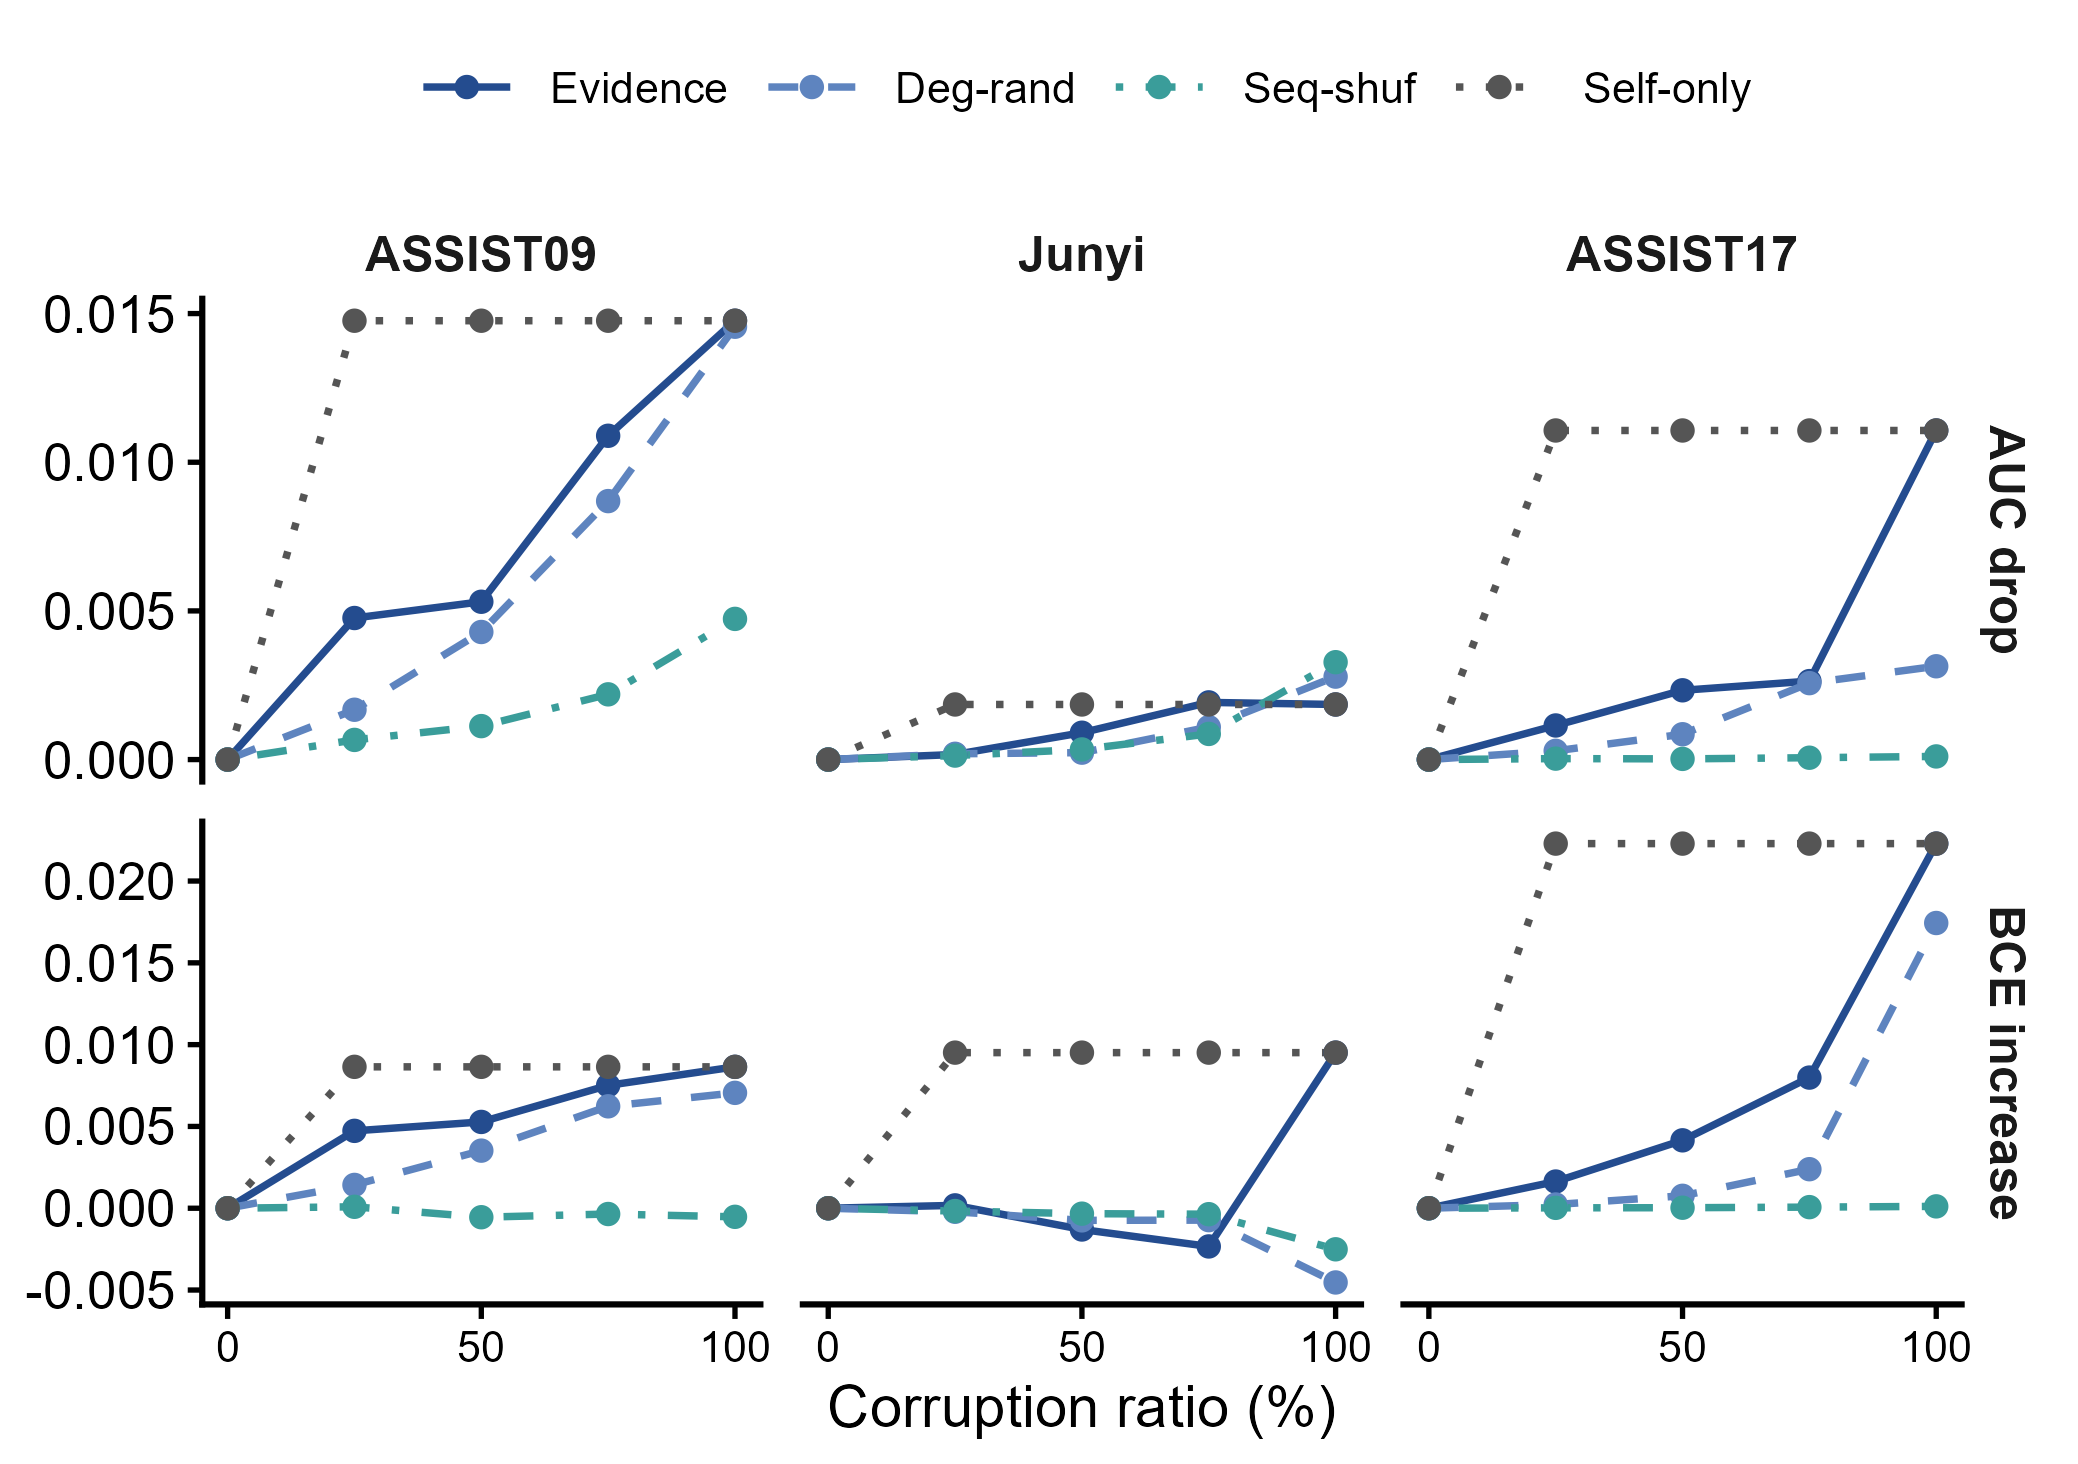
\includegraphics[width=0.98\columnwidth]{fig7_crg_support_perturbation.png}
  \caption{CRG support perturbation results. The upper row shows AUC drop and the lower row shows BCE increase under evidence corruption, degree-random support, sequence-shuffled support, and self-only fallback.}
  \label{fig:support-perturbation}
\end{figure}

Figure~\ref{fig:support-perturbation} shows that replacing CRG support changes prediction. ASSIST17 gives the clearest prediction-level support-dependence: evidence-supported replacement causes a larger degradation than degree-matched random replacement. ASSIST09 indicates sensitivity to the candidate support space, while Junyi shows a smaller AUC change and is not used as the main perturbation evidence.

This result complements concept retrieval from the prediction side. Retrieval shows that training-stage relations can recover plausible concept routes; perturbation shows that changing those support concepts can affect the trained model. The dataset-specific behavior suggests that CRG should be interpreted as training-log-constrained concept support rather than a curriculum graph.

\subsection{Learner-State Counterfactual and Same-Query Case}
CRG provides the support set, but LCRF determines how strongly each support concept contributes for a particular learner. We therefore use no-filter, mean-state, and shuffle-state variants to test whether the learner-state signal matters.

\begin{figure}[H]
  \centering
  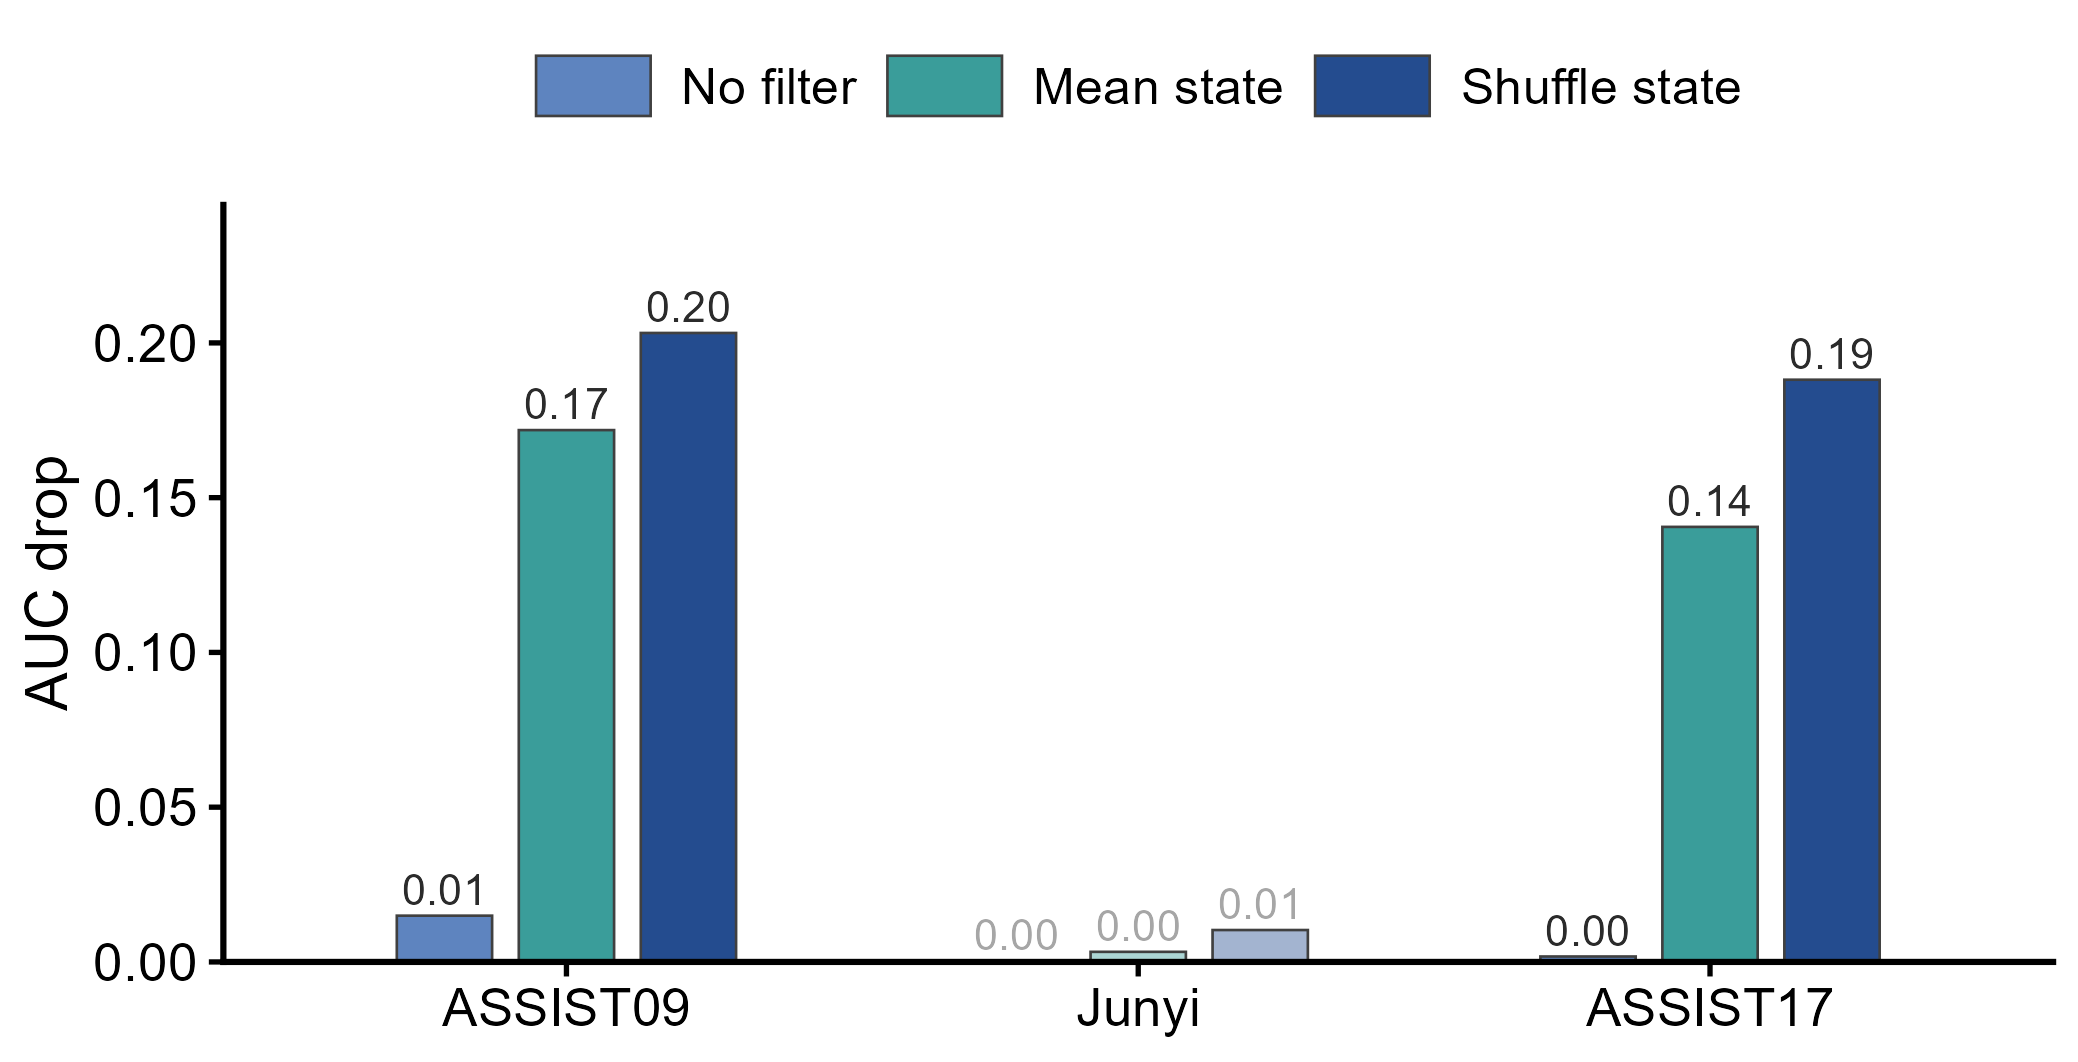
\includegraphics[width=0.98\columnwidth]{fig9_lcrf_counterfactual.png}
  \caption{Learner-state counterfactual results. Mean-state and shuffle-state replacement causes larger AUC drops on ASSIST09 and ASSIST17, while Junyi shows smaller changes and is treated as a route-construction-dominant case.}
  \label{fig:counterfactual}
\end{figure}

Figure~\ref{fig:counterfactual} distinguishes module removal from state replacement. Mean-state and shuffle-state variants cause clear degradation on ASSIST09 and ASSIST17, indicating that posterior weights depend on learner state. Junyi remains in the figure as a comparison case: its small drops suggest that the route-construction effect is more visible than learner-state filtering in this dataset.

\begin{figure}[H]
  \centering
  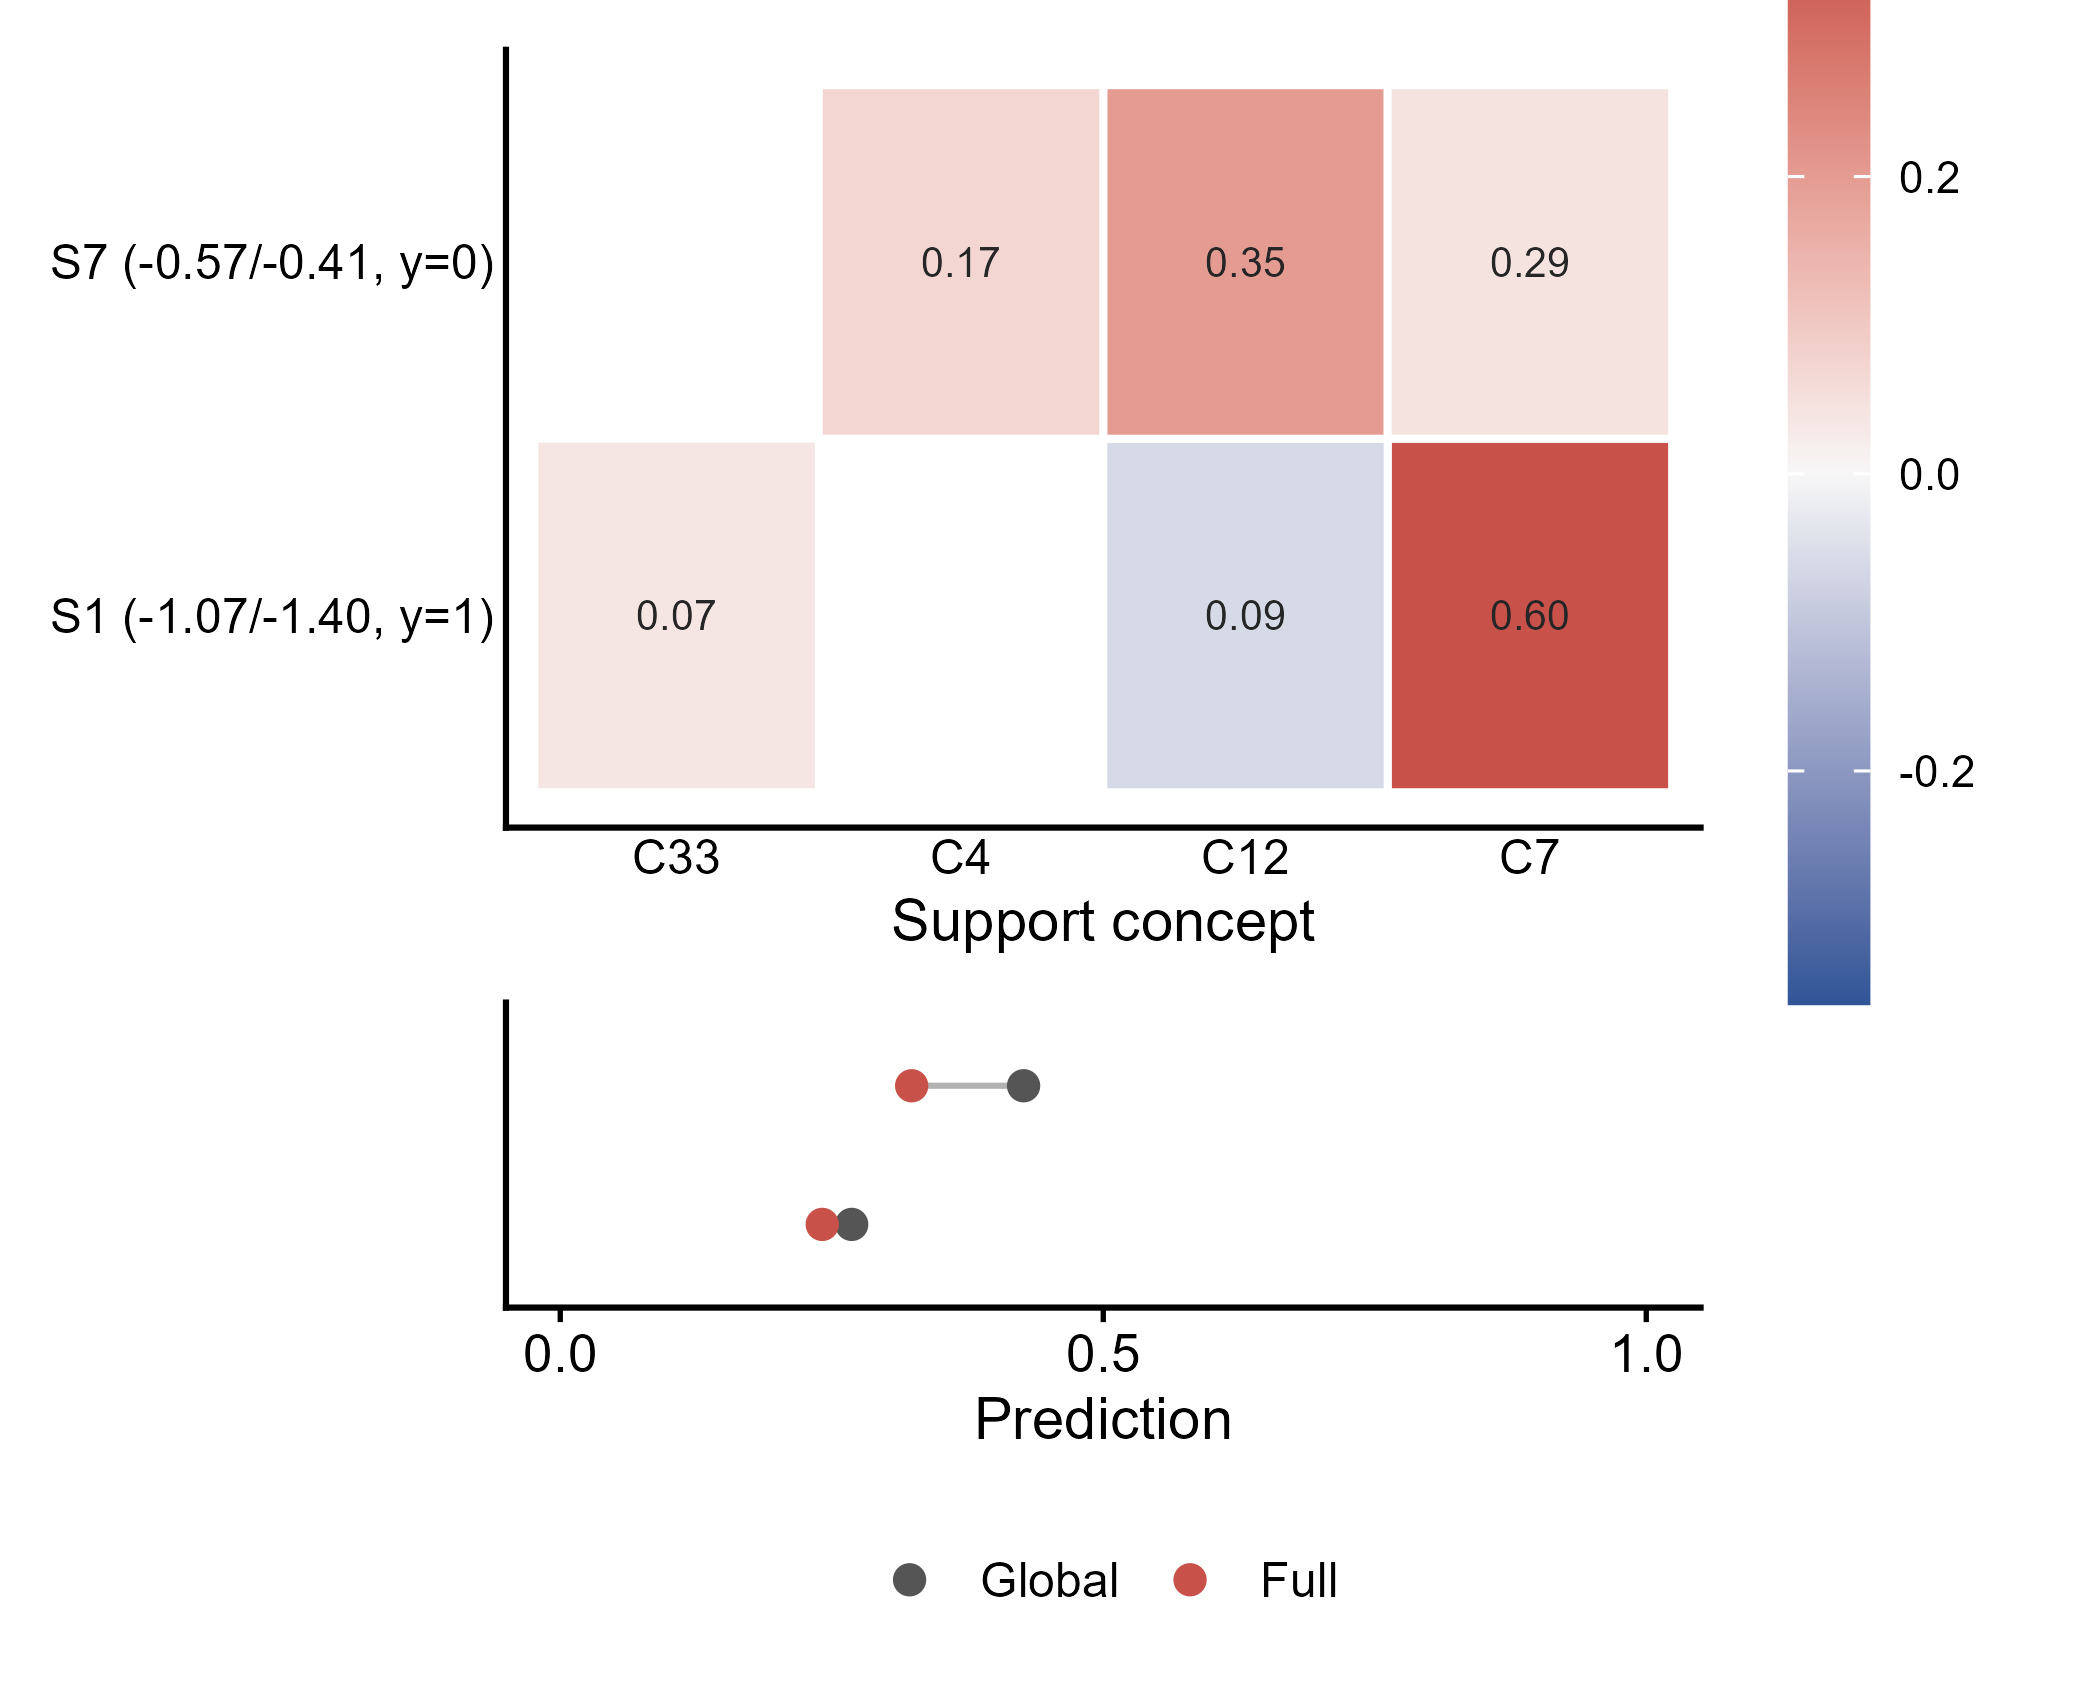
\includegraphics[width=0.98\columnwidth]{fig10_lcrf_same_query.png}
  \caption{Same-query posterior case. Under the same query concept and the same CRG support, different learners receive different posterior weights over support concepts.}
  \label{fig:same-query}
\end{figure}

Figure~\ref{fig:same-query} visualizes learner-conditioned filtering. Under the same query and the same CRG support, S1 assigns higher posterior weight to C7, while S7 emphasizes C12. LCRF therefore adapts support-concept weights within fixed support for different learners.

This case gives the learner-side interpretation of LCRF. CRG provides globally available support candidates, whereas LCRF selects among them according to mastery, recent performance, and historical counts. The selected cases show posterior shifts that co-vary with support-concept state variables: the strongest ASSIST09 case has positive association with support mastery and support count, while the ASSIST17 case shows a different state pattern under the same fixed-support constraint. We therefore use same-query cases to explain learner-conditioned filtering at the case level.

\section{Limitations}
The sequence relations in this work are empirical transitions from training logs rather than curriculum rules. They provide training-log-constrained route support, but they should not be interpreted as causal curriculum relations. This boundary is expected in educational diagnosis, because direct observations of the target concept remain the most specific signal when they are available. In addition, CRG-LCRF complements direct target-concept observations rather than replacing them. When sufficient direct observations on the target concept exist, the target-concept state remains an important signal. Future work can incorporate curriculum metadata, expert concept maps, richer learner-state sources, and causal route validation to better separate empirical transitions, curriculum structure, and learner-specific support.

\section{Conclusion}
We proposed CRG-LCRF for cognitive diagnosis under concept evidence gaps. CRG constructs a training-log-derived concept roadmap from item co-occurrence, sequence transition, and self-retention relations, and returns a fixed support set for each target concept. LCRF assigns learner-conditioned posterior weights over that support using mastery, recent performance, and historical counts. Experiments on three datasets show competitive prediction performance, target-concept retrieval from learner histories on selected datasets, and coverage-conditioned gains in subgroups where direct concept coverage is limited but candidate support exists. Support perturbation, learner-state counterfactuals, and same-query cases further illustrate how route support and learner-conditioned filtering affect prediction. These results provide an explicit route-support view for cognitive diagnosis when direct historical coverage of the target concept is limited.

\bibliographystyle{IEEEtran}
\bibliography{references_crg_lcrf}

\end{document}






